% Options for packages loaded elsewhere
\PassOptionsToPackage{unicode}{hyperref}
\PassOptionsToPackage{hyphens}{url}
%
\documentclass[
]{article}
\usepackage{amsmath,amssymb}
\usepackage{lmodern}
\usepackage{iftex}
\ifPDFTeX
  \usepackage[T1]{fontenc}
  \usepackage[utf8]{inputenc}
  \usepackage{textcomp} % provide euro and other symbols
\else % if luatex or xetex
  \usepackage{unicode-math}
  \defaultfontfeatures{Scale=MatchLowercase}
  \defaultfontfeatures[\rmfamily]{Ligatures=TeX,Scale=1}
\fi
% Use upquote if available, for straight quotes in verbatim environments
\IfFileExists{upquote.sty}{\usepackage{upquote}}{}
\IfFileExists{microtype.sty}{% use microtype if available
  \usepackage[]{microtype}
  \UseMicrotypeSet[protrusion]{basicmath} % disable protrusion for tt fonts
}{}
\makeatletter
\@ifundefined{KOMAClassName}{% if non-KOMA class
  \IfFileExists{parskip.sty}{%
    \usepackage{parskip}
  }{% else
    \setlength{\parindent}{0pt}
    \setlength{\parskip}{6pt plus 2pt minus 1pt}}
}{% if KOMA class
  \KOMAoptions{parskip=half}}
\makeatother
\usepackage{xcolor}
\usepackage[margin=1in]{geometry}
\usepackage{color}
\usepackage{fancyvrb}
\newcommand{\VerbBar}{|}
\newcommand{\VERB}{\Verb[commandchars=\\\{\}]}
\DefineVerbatimEnvironment{Highlighting}{Verbatim}{commandchars=\\\{\}}
% Add ',fontsize=\small' for more characters per line
\usepackage{framed}
\definecolor{shadecolor}{RGB}{248,248,248}
\newenvironment{Shaded}{\begin{snugshade}}{\end{snugshade}}
\newcommand{\AlertTok}[1]{\textcolor[rgb]{0.94,0.16,0.16}{#1}}
\newcommand{\AnnotationTok}[1]{\textcolor[rgb]{0.56,0.35,0.01}{\textbf{\textit{#1}}}}
\newcommand{\AttributeTok}[1]{\textcolor[rgb]{0.77,0.63,0.00}{#1}}
\newcommand{\BaseNTok}[1]{\textcolor[rgb]{0.00,0.00,0.81}{#1}}
\newcommand{\BuiltInTok}[1]{#1}
\newcommand{\CharTok}[1]{\textcolor[rgb]{0.31,0.60,0.02}{#1}}
\newcommand{\CommentTok}[1]{\textcolor[rgb]{0.56,0.35,0.01}{\textit{#1}}}
\newcommand{\CommentVarTok}[1]{\textcolor[rgb]{0.56,0.35,0.01}{\textbf{\textit{#1}}}}
\newcommand{\ConstantTok}[1]{\textcolor[rgb]{0.00,0.00,0.00}{#1}}
\newcommand{\ControlFlowTok}[1]{\textcolor[rgb]{0.13,0.29,0.53}{\textbf{#1}}}
\newcommand{\DataTypeTok}[1]{\textcolor[rgb]{0.13,0.29,0.53}{#1}}
\newcommand{\DecValTok}[1]{\textcolor[rgb]{0.00,0.00,0.81}{#1}}
\newcommand{\DocumentationTok}[1]{\textcolor[rgb]{0.56,0.35,0.01}{\textbf{\textit{#1}}}}
\newcommand{\ErrorTok}[1]{\textcolor[rgb]{0.64,0.00,0.00}{\textbf{#1}}}
\newcommand{\ExtensionTok}[1]{#1}
\newcommand{\FloatTok}[1]{\textcolor[rgb]{0.00,0.00,0.81}{#1}}
\newcommand{\FunctionTok}[1]{\textcolor[rgb]{0.00,0.00,0.00}{#1}}
\newcommand{\ImportTok}[1]{#1}
\newcommand{\InformationTok}[1]{\textcolor[rgb]{0.56,0.35,0.01}{\textbf{\textit{#1}}}}
\newcommand{\KeywordTok}[1]{\textcolor[rgb]{0.13,0.29,0.53}{\textbf{#1}}}
\newcommand{\NormalTok}[1]{#1}
\newcommand{\OperatorTok}[1]{\textcolor[rgb]{0.81,0.36,0.00}{\textbf{#1}}}
\newcommand{\OtherTok}[1]{\textcolor[rgb]{0.56,0.35,0.01}{#1}}
\newcommand{\PreprocessorTok}[1]{\textcolor[rgb]{0.56,0.35,0.01}{\textit{#1}}}
\newcommand{\RegionMarkerTok}[1]{#1}
\newcommand{\SpecialCharTok}[1]{\textcolor[rgb]{0.00,0.00,0.00}{#1}}
\newcommand{\SpecialStringTok}[1]{\textcolor[rgb]{0.31,0.60,0.02}{#1}}
\newcommand{\StringTok}[1]{\textcolor[rgb]{0.31,0.60,0.02}{#1}}
\newcommand{\VariableTok}[1]{\textcolor[rgb]{0.00,0.00,0.00}{#1}}
\newcommand{\VerbatimStringTok}[1]{\textcolor[rgb]{0.31,0.60,0.02}{#1}}
\newcommand{\WarningTok}[1]{\textcolor[rgb]{0.56,0.35,0.01}{\textbf{\textit{#1}}}}
\usepackage{graphicx}
\makeatletter
\def\maxwidth{\ifdim\Gin@nat@width>\linewidth\linewidth\else\Gin@nat@width\fi}
\def\maxheight{\ifdim\Gin@nat@height>\textheight\textheight\else\Gin@nat@height\fi}
\makeatother
% Scale images if necessary, so that they will not overflow the page
% margins by default, and it is still possible to overwrite the defaults
% using explicit options in \includegraphics[width, height, ...]{}
\setkeys{Gin}{width=\maxwidth,height=\maxheight,keepaspectratio}
% Set default figure placement to htbp
\makeatletter
\def\fps@figure{htbp}
\makeatother
\setlength{\emergencystretch}{3em} % prevent overfull lines
\providecommand{\tightlist}{%
  \setlength{\itemsep}{0pt}\setlength{\parskip}{0pt}}
\setcounter{secnumdepth}{-\maxdimen} % remove section numbering
\ifLuaTeX
  \usepackage{selnolig}  % disable illegal ligatures
\fi
\IfFileExists{bookmark.sty}{\usepackage{bookmark}}{\usepackage{hyperref}}
\IfFileExists{xurl.sty}{\usepackage{xurl}}{} % add URL line breaks if available
\urlstyle{same} % disable monospaced font for URLs
\hypersetup{
  pdftitle={HDB\_Case\_Study},
  pdfauthor={gabriel},
  hidelinks,
  pdfcreator={LaTeX via pandoc}}

\title{HDB\_Case\_Study}
\author{gabriel}
\date{2023-01-31}

\begin{document}
\maketitle

\hypertarget{gabriels-capstone-project}{%
\subsection{Gabriel's Capstone
Project}\label{gabriels-capstone-project}}

In this project I will be taking a look at the pernicious effects of the
HDB's 99-year leasehold by quantifying the rate of intrinsic value
deterioration, not accounting for inflation or market conditions.

\hypertarget{contents}{%
\subsubsection{Contents}\label{contents}}

\begin{enumerate}
\def\labelenumi{\arabic{enumi}.}
\tightlist
\item
  Data Preparation
\item
  Analysis\\
\item
  Key Findings
\item
  Conclusion
\end{enumerate}

\begin{center}\rule{0.5\linewidth}{0.5pt}\end{center}

\hypertarget{data-preperation}{%
\paragraph{1. Data Preperation}\label{data-preperation}}

The data set used in this project can be found at
\url{https://data.gov.sg/dataset/resale-flat-prices}\\
This data is based on the date of registration for resale transactions
between Jan 2012 and Jan 2023. Firstly since the data from the source
splits the years up in 3 different files, we will have to append them
together with power query.

\begin{figure}
\centering
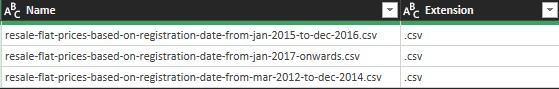
\includegraphics{images/process_append.jpeg}
\caption{Fig.1 Appending all 3 files together}
\end{figure}

The next step is to calculate the Remaining Lease of each unit at the
time of transaction. Which is given by the equation:
\[RL =  99 - (Y_{1} - Y_{0}) \]

\begin{itemize}
\tightlist
\item
  Where;

  \begin{itemize}
  \tightlist
  \item
    RL = Remaining Lease
  \item
    Y1 = Year transaction occurred
  \item
    Y2 = Year of lease commenced\\
  \end{itemize}
\end{itemize}

This is done with the following formula in Microsoft Excel:

\begin{verbatim}
=DATE(99-(YEAR([@month])-[@[lease_commence_date]]),MONTH([@month]),DAY([@month]))
\end{verbatim}

Now that we have prepared our data, let's get familiar with its contents
before we begin analysis.

\begin{Shaded}
\begin{Highlighting}[]
\FunctionTok{library}\NormalTok{(tidyverse)}
\end{Highlighting}
\end{Shaded}

\begin{verbatim}
## -- Attaching packages --------------------------------------- tidyverse 1.3.2 --
## v ggplot2 3.4.0      v purrr   0.3.5 
## v tibble  3.1.8      v dplyr   1.0.10
## v tidyr   1.2.1      v stringr 1.5.0 
## v readr   2.1.3      v forcats 0.5.2 
## -- Conflicts ------------------------------------------ tidyverse_conflicts() --
## x dplyr::filter() masks stats::filter()
## x dplyr::lag()    masks stats::lag()
\end{verbatim}

\begin{Shaded}
\begin{Highlighting}[]
\NormalTok{dataset }\OtherTok{\textless{}{-}} \FunctionTok{read.csv}\NormalTok{(}\StringTok{"Book1.csv"}\NormalTok{)}
\FunctionTok{glimpse}\NormalTok{(dataset)}
\end{Highlighting}
\end{Shaded}

\begin{verbatim}
## Rows: 234,765
## Columns: 11
## $ month               <chr> "03-2012", "03-2012", "03-2012", "03-2012", "03-20~
## $ town                <chr> "ANG MO KIO", "ANG MO KIO", "ANG MO KIO", "ANG MO ~
## $ flat_type           <chr> "2 ROOM", "2 ROOM", "3 ROOM", "3 ROOM", "3 ROOM", ~
## $ block               <chr> "172", "510", "610", "474", "604", "154", "110", "~
## $ street_name         <chr> "ANG MO KIO AVE 4", "ANG MO KIO AVE 8", "ANG MO KI~
## $ storey_range        <chr> "06 TO 10", "01 TO 05", "06 TO 10", "01 TO 05", "0~
## $ floor_area_sqm      <int> 45, 44, 68, 67, 67, 68, 67, 67, 67, 67, 68, 67, 68~
## $ flat_model          <chr> "Improved", "Improved", "New Generation", "New Gen~
## $ lease_commence_date <int> 1986, 1980, 1980, 1984, 1980, 1981, 1978, 1979, 19~
## $ remaining_lease     <int> 73, 67, 67, 71, 67, 68, 65, 66, 66, 72, 68, 67, 67~
## $ resale_price        <int> 250000, 265000, 315000, 320000, 321000, 321000, 32~
\end{verbatim}

\begin{Shaded}
\begin{Highlighting}[]
\FunctionTok{unique}\NormalTok{(dataset}\SpecialCharTok{$}\NormalTok{town)}
\end{Highlighting}
\end{Shaded}

\begin{verbatim}
##  [1] "ANG MO KIO"      "BEDOK"           "BISHAN"          "BUKIT BATOK"    
##  [5] "BUKIT MERAH"     "BUKIT PANJANG"   "BUKIT TIMAH"     "CENTRAL AREA"   
##  [9] "CHOA CHU KANG"   "CLEMENTI"        "GEYLANG"         "HOUGANG"        
## [13] "JURONG EAST"     "JURONG WEST"     "KALLANG/WHAMPOA" "MARINE PARADE"  
## [17] "PASIR RIS"       "PUNGGOL"         "QUEENSTOWN"      "SEMBAWANG"      
## [21] "SENGKANG"        "SERANGOON"       "TAMPINES"        "TOA PAYOH"      
## [25] "WOODLANDS"       "YISHUN"
\end{verbatim}

The output above shows the 11 columns that we're working with and the
234,765 transactions that make up this data set. Each one of these
transactions come from one of the 26 housing estates as seen above.

\hypertarget{analysis}{%
\paragraph{2. Analysis}\label{analysis}}

One might be tempted to assume a linear rate of deterioration in
property value, trending toward zero. However that is not the case, the
typical HDB's value follows the proverbial Bala's Curve (Fig.2). The
property value is a concave downward graph that exponentially decreases
it value the lower the tenure left.
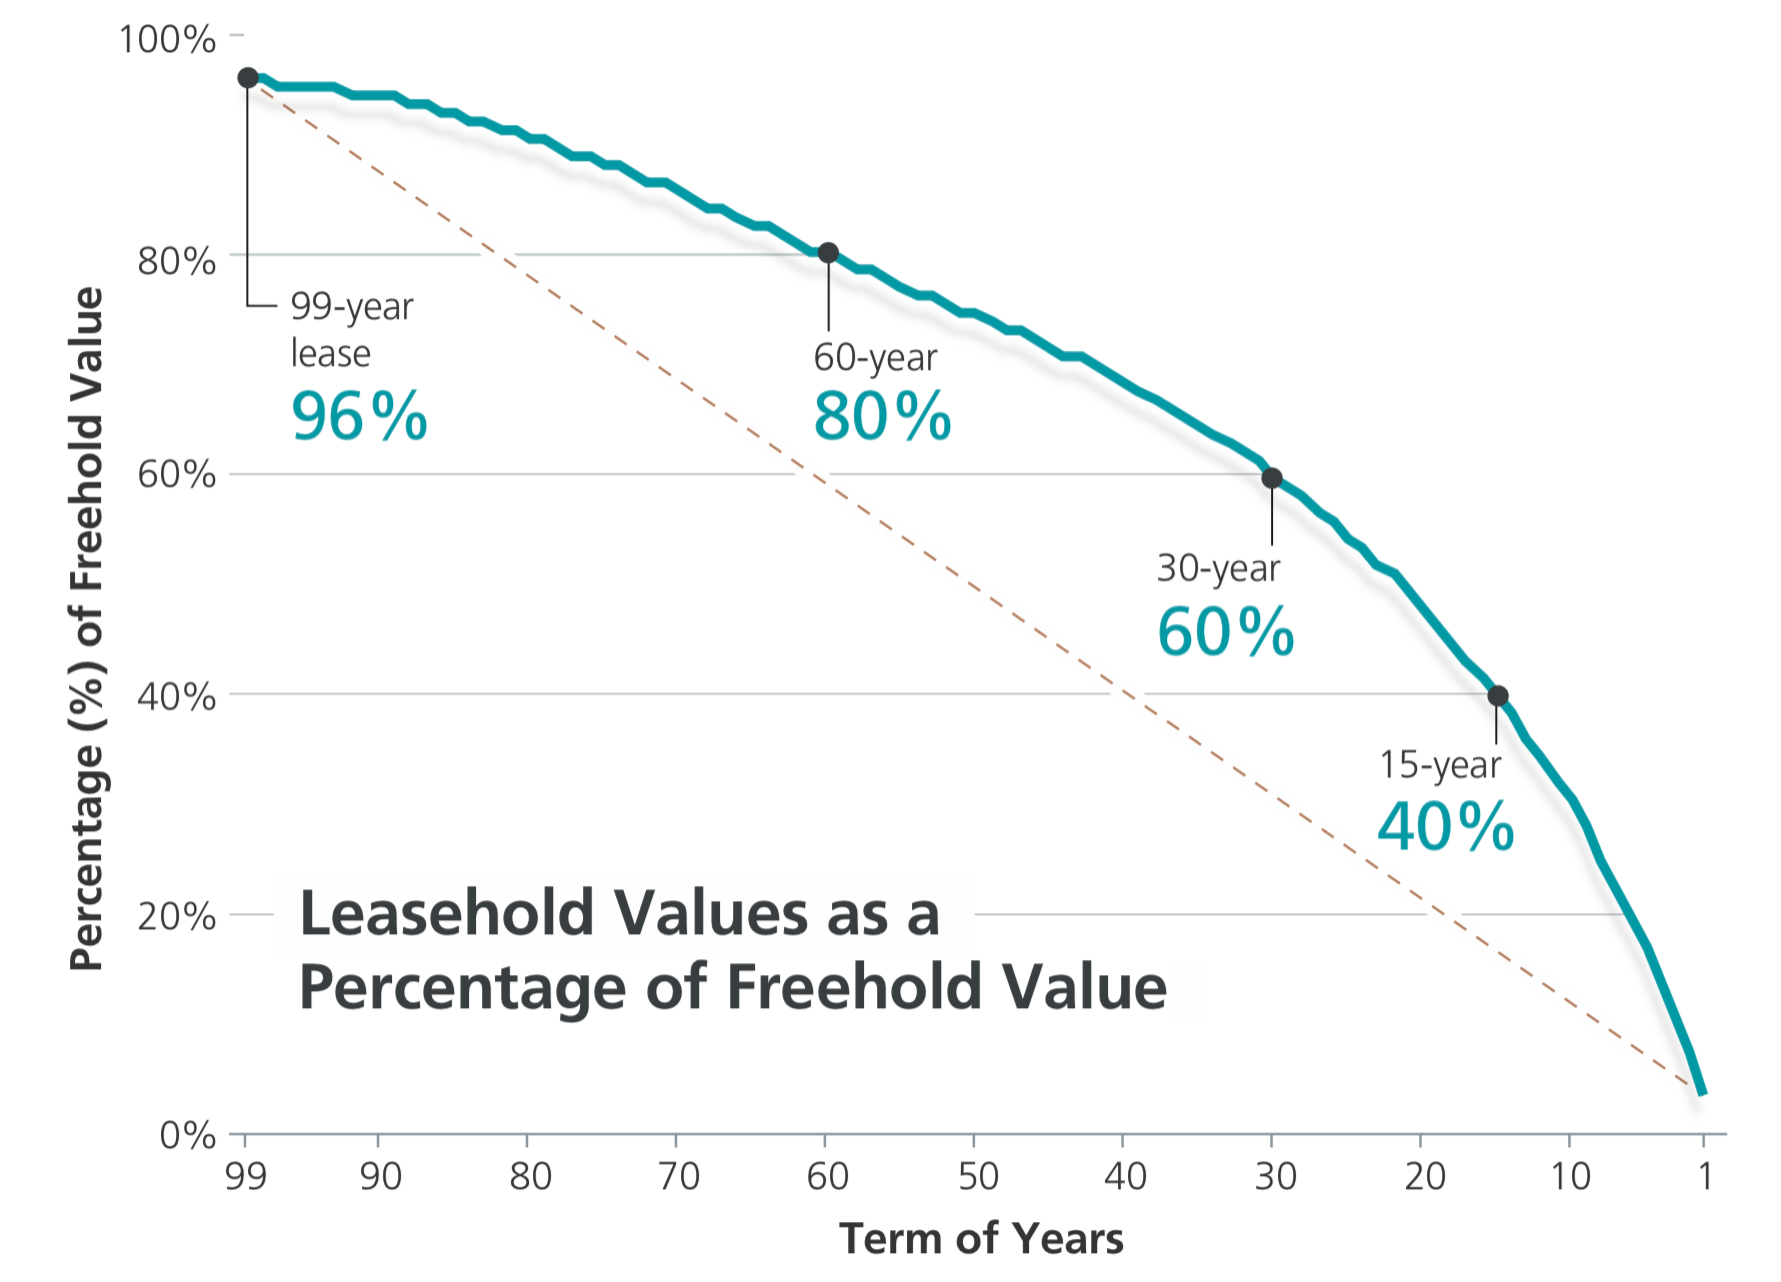
\includegraphics{images/Bala-curve.png}

From our data set let's find out the \emph{average} deterioration of
value by creating a linear model based on the covariance between resale
price and the remaining lease. Next we import the ``Broom'' package to
convert statistical analysis objects into tidy tibbles, we need this to
save the estimated regression value into the slope variable.

\begin{Shaded}
\begin{Highlighting}[]
\NormalTok{price\_model }\OtherTok{=} \FunctionTok{lm}\NormalTok{(resale\_price }\SpecialCharTok{\textasciitilde{}}\NormalTok{ remaining\_lease , }\AttributeTok{data =}\NormalTok{ dataset)}
\FunctionTok{summary}\NormalTok{(price\_model)}
\end{Highlighting}
\end{Shaded}

\begin{verbatim}
## 
## Call:
## lm(formula = resale_price ~ remaining_lease, data = dataset)
## 
## Residuals:
##     Min      1Q  Median      3Q     Max 
## -362166 -100340  -34674   66133  906748 
## 
## Coefficients:
##                  Estimate Std. Error t value Pr(>|t|)    
## (Intercept)     147214.77    1791.11   82.19   <2e-16 ***
## remaining_lease   4280.74      23.61  181.28   <2e-16 ***
## ---
## Signif. codes:  0 '***' 0.001 '**' 0.01 '*' 0.05 '.' 0.1 ' ' 1
## 
## Residual standard error: 143200 on 234763 degrees of freedom
## Multiple R-squared:  0.1228, Adjusted R-squared:  0.1228 
## F-statistic: 3.286e+04 on 1 and 234763 DF,  p-value: < 2.2e-16
\end{verbatim}

\begin{Shaded}
\begin{Highlighting}[]
\FunctionTok{library}\NormalTok{(broom)}
\NormalTok{price\_model }\SpecialCharTok{\%\textgreater{}\%} 
  \FunctionTok{tidy}\NormalTok{() }\SpecialCharTok{\%\textgreater{}\%} 
  \FunctionTok{filter}\NormalTok{(term }\SpecialCharTok{==} \StringTok{"remaining\_lease"}\NormalTok{) }\SpecialCharTok{\%\textgreater{}\%} 
  \FunctionTok{pull}\NormalTok{(estimate) }\OtherTok{{-}\textgreater{}}\NormalTok{ slope}
\end{Highlighting}
\end{Shaded}

Now that we have the slope variable we can pass this into our line plot
as an annotation.

\begin{Shaded}
\begin{Highlighting}[]
\NormalTok{dataset }\SpecialCharTok{\%\textgreater{}\%} 
  \FunctionTok{filter}\NormalTok{() }\SpecialCharTok{\%\textgreater{}\%} 
  \FunctionTok{ggplot}\NormalTok{(}\FunctionTok{aes}\NormalTok{(}\AttributeTok{x =} \FunctionTok{factor}\NormalTok{(remaining\_lease), }\AttributeTok{y =}\NormalTok{ resale\_price, }\AttributeTok{group =} \DecValTok{1}\NormalTok{)) }\SpecialCharTok{+}
  \FunctionTok{geom\_line}\NormalTok{(}\AttributeTok{stat =} \StringTok{\textquotesingle{}summary\textquotesingle{}}\NormalTok{, }\AttributeTok{fun =} \StringTok{\textquotesingle{}mean\textquotesingle{}}\NormalTok{) }\SpecialCharTok{+}
  \FunctionTok{geom\_smooth}\NormalTok{(}\AttributeTok{method =} \StringTok{\textquotesingle{}lm\textquotesingle{}}\NormalTok{)}\SpecialCharTok{+}
  \FunctionTok{labs}\NormalTok{(}\AttributeTok{title =} \StringTok{"Relationship between resale prices and lease tenure"}\NormalTok{)}\SpecialCharTok{+}
  \FunctionTok{annotate}\NormalTok{(}\StringTok{"text"}\NormalTok{, }\AttributeTok{x =}\DecValTok{20}\NormalTok{, }\AttributeTok{y=} \DecValTok{600000}\NormalTok{ ,}\AttributeTok{label=}\NormalTok{ (}\FunctionTok{paste0}\NormalTok{(}\StringTok{"Slope =="}\NormalTok{, slope)), }\AttributeTok{parse =} \ConstantTok{TRUE}\NormalTok{ )}
\end{Highlighting}
\end{Shaded}

\begin{verbatim}
## `geom_smooth()` using formula = 'y ~ x'
\end{verbatim}

\includegraphics{HDB_Case_Study_files/figure-latex/unnamed-chunk-3-1.pdf}

\hypertarget{key-findingssd}{%
\subsection{3. Key Findingssd}\label{key-findingssd}}

\end{document}
